\chapter{System Design and Architecture}

\section{Introduction}

This chapter presents a technical framework and architecture for implementing an embedded self-documenting DSL that is written in Scheme.  The proposed DSL provides human-friendly syntax that allows a user to select tables from a SQL database, translate them into RDF, and save the output in a specified file, all while generating a markdown file that has documentation about that given transformation.  Given the DSL's foundation in Scheme, end users are also able to leverage Scheme's capabilities within the DSL's framework, thereby enhancing its extensibility.

\section{Design Process}

\subsection{Design Goals}

In contrast to general-purpose languages (GPLs), DSLs present certain benefits, as highlighted by \citet{freudenthal2010domain} and \citet{spinellis2001notable}:

\begin{enumerate}
\item \textit{Explicit Representation of Domain Knowledge:} DSLs allow domain-specific functionality to be expressed in a tangible, human-readable format at a high level of abstraction.  This clarity makes software artifacts more accessible to developers, thereby simplifying the processes of development, testing and modification.
\item \textit{Active Engagement of Domain Experts:} Programs crafted in DSL often adopt a style that aligns with the conventional formats used by domain experts.  This facilitates their participation in the software's lifecycle and promotes collaboration with developers. In some cases, domain experts might directly specify, implement, verify or validate certain artifacts.
\end{enumerate}

In lieu of the aforementioned advantages of a DSL, the system architecture should accomplish the following:

\begin{enumerate}
\item The architecture must be \textit{database agnostic.}  Given that users will be employing this DSL with their unique databases, it is essential for the DSL to be flexible enough to support constructs that allows them to work with their unique database.
\item The architecture should empower users to model, in the context of some defined ontology, the mapping of the results derived from their SQL queries into RDF.
\item The DSL should provide a means of self-documenting itself while transforming data from SQL to RDF.
\end{enumerate}

\subsection{Architecture}
% How did you design your system
\begin{figure}[H]
  \centering
  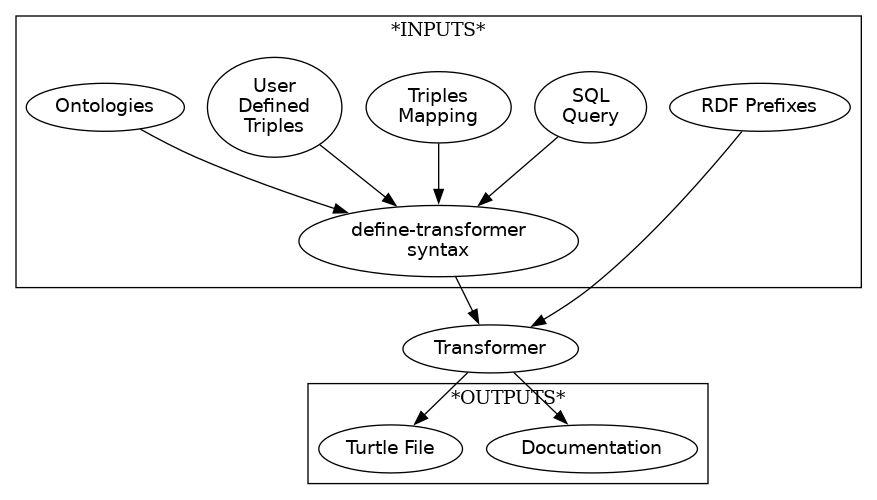
\includegraphics[width=12cm]{systemDesign}
  \caption{\textit{Overview of how SQL is converted to RDF and documentation}}
  \label{fig:system-diagram}
  \centering
\end{figure}

Figure \ref{fig:system-diagram} shows the overarching structure of the DSL under consideration.  In general, the transformation from SQL to RDF comprises the processing of distinct input components into a set of outputs: a turtle and markdown file.  These inputs comprise:

\begin{enumerate}
\item \textit{Ontologies}: An ontology is a formal way of representing knowledge.  In the context of Genenetwork, several ontologies are selected to server as conceptual frameworks for characterizing various entities, including experiments, investigators, species, genes and other relevant entities.
\item \textit{SQL Query}: Acting as the most important instruction set, the SQL query is executed as a pivotal step in the transformation process.
\item \textit{Triples Mapping}: This is a clear mapping between the results of the aforementioned SQL query and the corresponding RDF structure.
\item \textit{User Defined Triples}: In scenarios where existing ontologies fail to encompass domain-specific concepts within the Genenetwork context, user-defined triples are introduced to accommodate these unique conceptual dimensions.
\item \textit{RDF Prefixes}: These are the RDF namespaces that will be appended to the beginning of the turtle file.
\end{enumerate}

The ``define-transformer'' macro is the central driver for converting SQL to RDF.  It provides an interface for specifying the SQL query, user-defined triples, and SQL-to-RDF mapping. The ``define-transformer'' macro is one of the inputs to the ``transform-with-documentation'' macro which takes objects using the ``define-transformer'' macro as input, along with RDF prefixes. It then parses the abstract syntax tree of the ``define-transformer'' macro to automatically generate documentation, and executes the transformation itself, resulting in a Turtle file.

%%% Local Variables:
%%% ispell-local-dictionary: "en_GB-ise"
%%% End:
